\documentclass[11pt]{article}

% ---------- Page & fonts ----------
\usepackage[margin=1in]{geometry}
\usepackage[utf8]{inputenc}
\usepackage[T1]{fontenc}

% ---------- Math ----------
\usepackage{amsmath, amssymb, amsthm, mathtools}

% ---------- Graphs / figures ----------
\usepackage{tikz}
\usetikzlibrary{positioning, arrows.meta, calc}

% ---------- Quality of life ----------
\usepackage{enumitem}
\usepackage{hyperref}
\usepackage{cleveref}
\usepackage{xcolor}

\hypersetup{
  colorlinks=true,
  linkcolor=blue!50!black,
  citecolor=blue!50!black,
  urlcolor=blue!50!black
}

% ================= Theorem environments =================
\theoremstyle{plain}
\newtheorem{theorem}{Theorem}[section]
\newtheorem{lemma}[theorem]{Lemma}
\newtheorem{proposition}[theorem]{Proposition}
\newtheorem{corollary}[theorem]{Corollary}
\newtheorem{conjecture}[theorem]{Conjecture}

\theoremstyle{definition}
\newtheorem{definition}[theorem]{Definition}
\newtheorem{example}[theorem]{Example}
\newtheorem{exercise}[theorem]{Exercise}

\theoremstyle{remark}
\newtheorem{remark}[theorem]{Remark}
\newtheorem*{note}{Note}

% ================= Graph theory macros =================
% Sets
\newcommand{\V}{V}                       % vertex set
\newcommand{\E}{E}                       % edge set
\newcommand{\N}{N}                       % neighbourhood, N(v)

% Common graph families
\newcommand{\Kn}[1]{K_{#1}}              % complete graph K_n
\newcommand{\Kmn}[2]{K_{#1,#2}}          % complete bipartite K_{m,n}
\newcommand{\Cn}[1]{C_{#1}}              % cycle
\newcommand{\Pn}[1]{P_{#1}}              % path

% Invariants (as operators, upright text, correct spacing)
\DeclareMathOperator{\dg}{d}             % degree, use dg(v) to avoid clashing with \deg
\DeclareMathOperator{\ex}{ex}            % extremal function ex(n, H)
\DeclareMathOperator{\girth}{girth}
\DeclareMathOperator{\diam}{diam}
\DeclareMathOperator{\Aut}{Aut}
\DeclareMathOperator{\chr}{\chi}          % chromatic number, use \chr(G)
\DeclareMathOperator{\comp}{c}            % number of components

% Misc shorthands
\newcommand{\iso}{\cong}                 % isomorphic
\newcommand{\subgraph}{\subseteq}        % spanning/sub relations, adjust as needed

% ================= TikZ Styles =================
\tikzset{
    vertex/.style={
        circle,
        draw=black,
        fill=black,
        inner sep=1.8pt
    },
    edge/.style={
        thick
    },
    rededge/.style={
        thick,
        red
    },
    blueedge/.style={
        thick,
        blue
    }
}

% ================= Document =================
\title{Regular Graphs}
\author{Siddharth Narayan Mishra}
\date{\today}

\begin{document}

\maketitle

\begin{definition}[k-Regular Graph]
  A graph $G=(V,E)$ is called \textbf{$k$-regular} if every vertex has degree exactly $k$ neighbours. Formally,

  \[
    \deg(v)=k,\qquad \forall v\in V(G).
  \]

  That is, every vertex is incident to exactly $k$ edges.
\end{definition}

\bigskip

\begin{example}[1-Regular Graph]
  Every vertex has degree $1$. Such graphs consist of disjoint edges.

  \begin{center}
    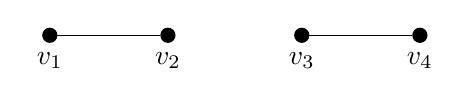
\begin{tikzpicture}[
        vertex/.style={circle,draw,fill=black,inner sep=1.8pt}
      ]

      \node[vertex,label=below:$v_1$] (A) at (0,0) {};
      \node[vertex,label=below:$v_2$] (B) at (1.5,0) {};
      \node[vertex,label=below:$v_3$] (C) at (3.2,0) {};
      \node[vertex,label=below:$v_4$] (D) at (4.7,0) {};

      \draw (A)--(B);
      \draw (C)--(D);

    \end{tikzpicture}
  \end{center}

  Each vertex is incident to exactly one edge.
\end{example}

\bigskip

\begin{example}[2-Regular Graph]
  Every vertex has degree $2$. A connected $2$-regular graph is a cycle.

  \begin{center}
    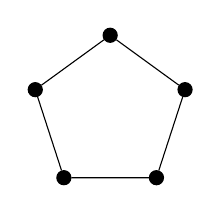
\begin{tikzpicture}[
        vertex/.style={circle,draw,fill=black,inner sep=1.8pt}
      ]

      \foreach \i/\x/\y in {
          1/90/1,
          2/18/1,
          3/-54/1,
          4/-126/1,
          5/-198/1}
        {
          \node[vertex] (v\i) at (\x:\y) {};
        }

      \draw (v1)--(v2)--(v3)--(v4)--(v5)--(v1);

    \end{tikzpicture}
  \end{center}

  Each vertex has two neighbours.
\end{example}

\bigskip

\begin{example}[3-Regular (Cubic) Graph]
  A graph is \textbf{3-regular} if every vertex has degree $3$.

  \begin{center}
    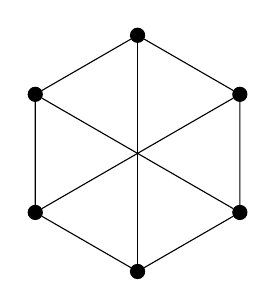
\begin{tikzpicture}[
        vertex/.style={circle,draw,fill=black,inner sep=1.8pt}
      ]

      \node[vertex] (A) at (90:1.5) {};
      \node[vertex] (B) at (150:1.5) {};
      \node[vertex] (C) at (210:1.5) {};
      \node[vertex] (D) at (270:1.5) {};
      \node[vertex] (E) at (330:1.5) {};
      \node[vertex] (F) at (30:1.5) {};

      \draw (A)--(B)--(C)--(D)--(E)--(F)--(A);
      \draw (A)--(D);
      \draw (B)--(E);
      \draw (C)--(F);

    \end{tikzpicture}
  \end{center}

  Every vertex is incident to exactly three edges.
\end{example}

\bigskip

\begin{definition}[$2k$-Regular Graph]
  A graph $G$ is said to be \textbf{$2k$-regular} if every vertex has even degree
  $2k$, i.e.,

  \[
    \deg(v)=2k,\qquad \forall v\in V(G).
  \]

  Examples include

  \[
    \begin{array}{c|c}
      k & \text{Graph Type} \\
      \hline
      1 & 2\text{-regular}  \\
      2 & 4\text{-regular}  \\
      3 & 6\text{-regular}  \\
      4 & 8\text{-regular}
    \end{array}
  \]
\end{definition}

\begin{remark}
  The paper focuses on $2k$-regular graphs because every vertex has even degree. This enables the application of \emph{Petersen's 2-Factor Theorem}, which states that every $2k$-regular graph can be decomposed into $k$ edge-disjoint $2$-factors. This decomposition is fundamental to the proofs developed later in the paper.
\end{remark}

\end{document}